\begin{frame}{lab: doubly-linked list}
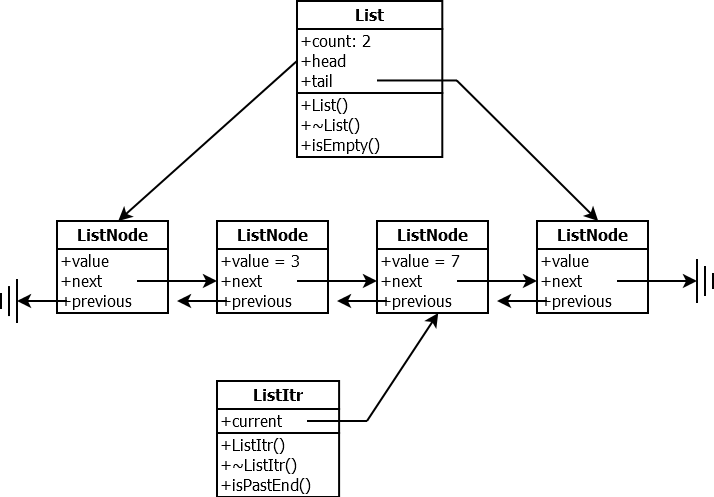
\includegraphics[height=0.9\textheight]{list-diagram}
\end{frame}

\begin{frame}[fragile,label=labListDecl]{the lab's list declaration}
\lstset{
    language=C++,
    style=small,
    moredelim={**[is][\btHL<all:2>]{@2}{2@}},
    moredelim={**[is][\btHL<all:3>]{@3}{3@}},
    moredelim={**[is][\btHL<all:4>]{@4}{4@}},
}
\begin{lstlisting}
class ListNode {

public:
    ListNode();                // Constructor
    ...
private:
    int value;
    @2ListNode *next, *previous2@;

    @3friend class List;3@
    @4friend class ListItr;4@
};
\end{lstlisting}
\begin{tikzpicture}[overlay,remember picture]
\coordinate (place) at ([yshift=4cm]current page.south);
\tikzset{
    markBox/.style={draw=red,very thick,align=left,at=(place), fill=white},
}
\begin{visibleenv}<2>
\node[markBox] {\texttt{*} binds to name --- declares two pointers; \\
                (why I write \texttt{*} next to names)};
\end{visibleenv}
\begin{visibleenv}<3>
\node[markBox] {the class \texttt{List} can access \\ private members of \texttt{ListNode}};
\end{visibleenv}
\begin{visibleenv}<4>
\node[markBox] {the class \texttt{ListItr} can access \\ private members of \texttt{ListNode}};
\end{visibleenv}
\end{tikzpicture}
\end{frame}

\begin{frame}[fragile,label=labListLocal1]{a common mistake (1)}
\lstset{
    language=C++,
    style=small,
    moredelim={**[is][\btHL<all:2>]{@2}{2@}},
    moredelim={**[is][\btHL<all:3>]{@3}{3@}},
    moredelim={**[is][\btHL<all:4>]{@4}{4@}},
}
\begin{lstlisting}
class Foo {
public:
  Foo();
private:
  ListNode *@2head2@;
  ...
};
Foo::Foo() {
  ListNode *@2head2@ = new ListNode; // BROKEN!
}
\end{lstlisting}
\begin{itemize}
\item what's wrong with this?
\end{itemize}
\begin{tikzpicture}[overlay,remember picture]
    \tikzset{
        >=Latex,
        dealloced/.style={alt=<4->{opacity=0.25}}
    }
\coordinate (place) at ([yshift=7.5cm,xshift=0cm]current page.south);
\begin{visibleenv}<2->
\node[draw,font=\tt,thick,anchor=north west,label={north:Foo object},minimum width=2cm] (fooHead) at (place) {
    head
};
\node[draw,font=\tt,thick,anchor=north west,minimum width=2cm] (fooRest) at (fooHead.south west) {\ldots};
    \node[draw,font=\tt,thick,anchor=north west,label={north:local variables},minimum width=2cm] (fooLocal) at ([yshift=-2.5cm]place) {
    head
};
\end{visibleenv}
\begin{visibleenv}<3->
    \node[right=1.5cm of fooHead,thick,label={north:ListNode},rectangle split,rectangle split parts=3,draw] (fooNode) {
    next
    \nodepart{second} prev
    \nodepart{third} \ldots
};
    \draw[ultra thick,red,->] (fooLocal) -- ++(2cm,0cm) |- ([yshift=-.25cm]fooNode.north west);
\end{visibleenv}
\end{tikzpicture}
\end{frame}



\begin{frame}[fragile,label=labListLocal2]{a common mistake (2)}
\lstset{
    language=C++,
    style=small,
    moredelim={**[is][\btHL<all:2>]{@2}{2@}},
    moredelim={**[is][\btHL<all:3>]{@3}{3@}},
    moredelim={**[is][\btHL<all:4>]{@4}{4@}},
}
\begin{lstlisting}
class Foo {
public:
  Foo();
private:
  ListNode *@2head2@;
  ...
};
Foo::Foo() {
  ListNode temp;
  head = @2&temp2@;
}
\end{lstlisting}
\begin{itemize}
\item what's wrong with this?
\end{itemize}
\begin{tikzpicture}[overlay,remember picture]
    \tikzset{
        >=Latex,
        dealloced/.style={alt=<4->{opacity=0.25}}
    }
\coordinate (place) at ([yshift=7.5cm,xshift=0cm]current page.south);
\begin{visibleenv}<2->
\node[draw,font=\tt,thick,anchor=north west,label={north:Foo object},minimum width=2cm] (fooHead) at (place) {
    head
};
\node[thick,rectangle split,rectangle split parts=3,draw,anchor=north west,
        label={[alias=fooNodeLabel,dealloced]north:{temp:}},dealloced] (fooNode)
        at ([xshift=.25cm,yshift=-3cm]place) {
    next
    \nodepart{second} prev
    \nodepart{third} \ldots
};
    \node[below=1mm of fooNode] (belowFooNode) {};
    \node[inner sep=0mm,inner xsep=1mm,fit=(fooNode) (fooNodeLabel) (belowFooNode),draw,thick,
        label={[dealloced]north:local variables},dealloced] {};
\end{visibleenv}
\begin{visibleenv}<3->
    \draw[ultra thick,red,->] (fooHead) -- ++(2cm,0cm) |- ([yshift=-.25cm]fooNode.north east);
\end{visibleenv}
\end{tikzpicture}
\end{frame}
